% ex: ts=2 sw=2 sts=2 et filetype=tex
% SPDX-License-Identifier: CC-BY-SA-4.0
\begin{frame}
    \frametitle{Contenido}
    \tableofcontents
\end{frame}

\section{Algoritmo y sus características}

\begin{frame}[c]{Algoritmo}
  \begin{columns}
    \column{0.7\textwidth}
    \begin{block}{Definición}
      \begin{itemize}
        \item Conjunto ordenado y finito de operaciones que permite hallar
              la solución de un problema\footnote{Real academia española}.
        \item Conjunto de pasos, acciones o instrucciones necesarios para
              lograr un resultado o resolver un problema.
      \end{itemize}
    \end{block}
    \column{0.3\textwidth}
    \begin{center}
    \begin{tikzpicture}[node distance = 1cm, node font=\tiny]
      \node (inicio) [iniciofin] {Inicio};
      \node (e1)   [entrada, below of=inicio] {Entrada};
      \node (proc1) [proceso, below of=e1] {Proceso 1};
      \node (dec1)  [decision, below of=proc1, yshift=-0.4cm] {Decisión};
      \node (proc2a) [proceso, below of=dec1,  yshift=-0.4cm] {Proceso 2a};
      \node (proc2b) [proceso, right of=dec1,  xshift=1.2cm] {Proceso 2b};
      \node (s1)   [salida, below of=proc2a] {Salida};
      \node (fin) [iniciofin, below of=s1] {fin};

      \draw[flecha] (inicio) -- (e1);
      \draw[flecha] (e1) -- (proc1);
      \draw[flecha] (proc1) -- (dec1);
      \draw[flecha] (dec1) -- node[anchor=east]{si} (proc2a);
      \draw[flecha] (dec1) -- node[anchor=south]{no}(proc2b);
      \draw[flecha] (proc2a) -- (s1);
      \draw[flecha] (s1) -- (fin);
      \draw[flecha] (proc2b) |- (s1);

    \end{tikzpicture}
    \end{center}
  \end{columns}
\end{frame}

\begin{frame}[c]{Algoritmo}
  \begin{columns}
    \column{0.7\textwidth}
    \begin{center}
      \begin{tikzpicture}[node distance = 2cm]
        \node (problema) [rectangle, fill=none]{Problema};
        \node (flecha) [single arrow, minimum height=1.5cm, right of=problema, fill=cyan!50]{};
        \node (solucion) [rectangle, fill=none, right of=flecha] {Solución};
      \end{tikzpicture}

      \vspace{1cm}

      \begin{itemize}
        \item El mismo problema puede ser resuelto por más de dos algoritmos
          diferentes. Mientras más grande sea el problema mayor es la diversidad
          de algoritmos que existen para resolverlo.
      \end{itemize}
    \end{center}
    \column{0.3\textwidth}
    \begin{center}
    \begin{tikzpicture}[node distance = 1cm, node font=\tiny]
      \node (inicio) [iniciofin] {Inicio};
      \node (e1)   [entrada, below of=inicio] {Entrada};
      \node (proc1) [proceso, below of=e1] {Proceso 1};
      \node (dec1)  [decision, below of=proc1, yshift=-0.4cm] {Decisión};
      \node (proc2a) [proceso, below of=dec1,  yshift=-0.4cm] {Proceso 2a};
      \node (proc2b) [proceso, right of=dec1,  xshift=1.2cm] {Proceso 2b};
      \node (s1)   [salida, below of=proc2a] {Salida};
      \node (fin) [iniciofin, below of=s1] {fin};

      \draw[flecha] (inicio) -- (e1);
      \draw[flecha] (e1) -- (proc1);
      \draw[flecha] (proc1) -- (dec1);
      \draw[flecha] (dec1) -- node[anchor=east]{si} (proc2a);
      \draw[flecha] (dec1) -- node[anchor=south]{no}(proc2b);
      \draw[flecha] (proc2a) -- (s1);
      \draw[flecha] (s1) -- (fin);
      \draw[flecha] (proc2b) |- (s1);

    \end{tikzpicture}
    \end{center}
  \end{columns}
\end{frame}

\begin{frame}[c]{Algoritmo}
  Los algoritmos pueden tener:

  \begin{columns}[t]
    \column{0.3\textwidth}
      \begin{center}
        \textbf{Operaciones} \\
        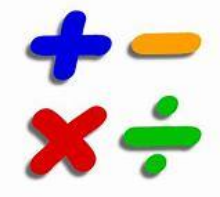
\includegraphics[scale=0.2]{010-operaciones.png}
      \end{center}
      Aritméticas, relacionales, lógicas, de lectura y escritura.

    \column{0.3\textwidth}
      \begin{center}
      \textbf{Decisiones} \\
        
\includegraphics[scale=0.2]{010-decisiones.png}
      \end{center}
      La ejecución de una instrucción puede depender del resultado de la
      instrucción anterior.

    \column{0.3\textwidth}
      \begin{center}
      \textbf{Repeticiones} \\
        
\includegraphics[scale=0.2]{010-repeticiones.png}
      \end{center}
      Un mismo bloque de instrucciones puede repetirse más de una vez para
      lograr el resultado esperado.
  \end{columns}
\end{frame}

\begin{frame}[c]{Características de un algoritmo}
  \begin{center}
    \begin{tabular}{c l}
      Ordenado & Las instrucciones se ejecutan una después de otra en un orden
      específico. Al cambiar el orden, puede cambiar el resultado. \\
      Finito & El algoritmo debe tener un inicio y un fin. \\
      Preciso & Cada vez que se ejecute el algoritmo usando los mismos datos
      de entrada, debe producir la misma salida. \\
      Definido & Cada instrucción atiende un solo problema particular. No se
      presta a ambigüedades (dobles significados).
    \end{tabular}

      
\begin{tikzpicture}[node distance = 2cm]
        \node [rectangle,rounded corners, shading=radial]{Ordenado};
      \end{tikzpicture}
      presta a ambigüedades (dobles significados).


  \end{center}
\end{frame}


\begin{frame}[c]{Características de un algoritmo}
  \smartdiagram[descriptive diagram]{
  {Ordenado, {Las instrucciones se ejecutan una después de otra en un orden
      específico. Al cambiar el orden, puede cambiar el resultado.}},
  {Finito, El algoritmo debe tener un inicio y un fin.},
  {Preciso, {Cada vez que se ejecute el algoritmo usando los mismos datos
      de entrada, debe producir la misma salida.}},
  {Definido,{Cada instrucción atiende un solo problema particular. No se
      presta a ambigüedades (dobles significados).}}}
\end{frame}




\section{Lenguajes de programación y su clasificación}

\begin{frame}[c]{Título}
    \begin{center}
        Texto
    \end{center}
\end{frame}
